\chapter{\IfLanguageName{dutch}{Opstellen ELK}{Opstellen ELK}}%
\label{ch:Opstellen ELK}
In dit hoofdstuk zal worden gekeken hoe er toegang tot ELK kan worden verleend aan MFPOSS en welke voorbereidingen we hiervoor moeten treffen. Het is niet de bedoeling ELK op de mainframe te installeren, aangezien Colruyt Group Services al ELK buiten de mainframe gebruikt en een team heeft dat het beheert.

\section{Opstellen ELK voor MFPOSS}
Het doel van dit onderzoek is om een prototype van een ELK-dashboard te kunnen leveren aan MFPOSS om te beoordelen of het aan de MoSCoW-eisen voldoet. Om dit te bereiken, moet eerst een contactpersoon worden gevonden bij ELK om te verkennen welke mogelijkheden er zijn om onze data naar ELK te sturen. Het eerste contact met ELK was met Anusha, zij is een medewerker in het OPMONTOOLS-team dat ELK beheert. Vanaf dit punt zullen ze worden aangeduid als het ELK-team. Voordat we doorgaan met het onderzoek, is het belangrijk om te weten of er mogelijkheden zijn om de SYSLOGS naar het ELK-team te sturen. Na een vergadering met Dieter en daarna met Anusha is snel geconcludeerd dat we de gegevens periodiek over TCP/IP kunnen verzenden. Er zijn vermoedens dat Filebeat hiervoor misschien ook kan worden gebruikt, indien nodig. Het besluit om gegevens te verzenden, moet worden genomen voordat ELK wordt opgezet, om onnodig werk te voorkomen. Zodra is besloten dat er een grote kans is om de logs succesvol naar ELK te kunnen sturen, is er een aanvraag ingediend om toegang te krijgen tot ELK. Deze aanvraag is ingediend via ServiceNow. Een verantwoordelijke van het ELK-team zal die aanvraag oppakken en ons verder helpen. Anusha heeft ook gemeld dat als er geen problemen zijn, we binnen tien dagen een integratie kunnen verwachten.

\subsection{Aanvragen ELK}
Zoals eerder besproken, is ServiceNow een platform waar Colruyt Group verschillende soorten tickets behandelt. Deze tickets zijn bedoeld om problemen op te lossen of zaken aan te vragen. Voor dit onderzoek is aanvragen van belang. Maar als er na dit onderzoek problemen optreden, kan contact opnemen met ServiceNow of een medewerker een mogelijke vervolgstap zijn. Het verzoek dat is ingediend, is hetzelfde verzoek dat kan worden bekeken in figuur 4.1. Laten we elk veld kort bespreken.

\begin{figure}
    \centering
    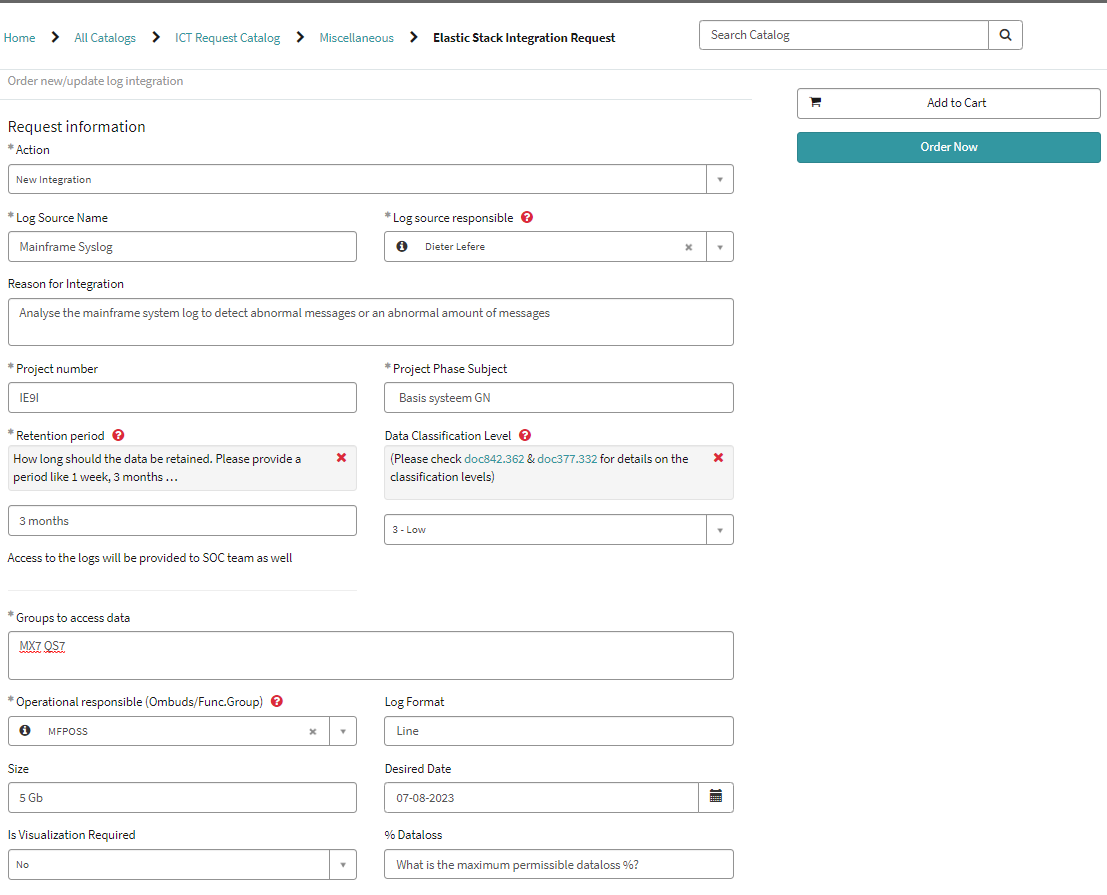
\includegraphics[width=1\linewidth]{bachproef//graphics/Request.png}
    \caption{Een verzoek voor een nieuwe ELK-integratie}
    \label{fig:Een ServiceNow-verzoek om een nieuwe ELK-integratie te starten}
\end{figure}

\subsubsection{Action}
Dit veld is verplicht en is een dropdown met twee opties. De opties zijn als volgt:
\begin{itemize}
    \item New Integration: Dit is om een nieuwe integratie van ELK aan te vragen. Dit is de optie die voor dit onderzoek zal worden gebruikt.
    \item Modify Integration: Deze optie kan worden gebruikt om bestaande ELK-integraties aan te passen.
\end{itemize}

\subsubsection{Log source name}
Dit is een verplicht veld. Hier moet een naam worden opgegeven voor de logs. Deze zullen onder deze naam in ELK verschijnen. Voor dit onderzoek is de waarde die we hier hebben gekozen "Mainframe Syslog."

\subsubsection{Log source responsible}
Dit verplichte veld dient om een medewerker van het team dat hun logs wil versturen aan te geven. Deze persoon wordt dan beschouwd als verantwoordelijk voor de logs. Voor MFPOSS is dit Dieter Lefere.

\subsubsection{Reason for integration}
Dit is een niet-verplicht veld waarin een korte uitleg kan worden gegeven waarom de ELK-integratie wordt aangevraagd. Dit is handig voor context, maar dit kan natuurlijk ook in latere vergaderingen worden besproken. Hier hebben we vermeld dat we de logs van het mainframesysteem willen bekijken om te zien hoe vaak hetzelfde bericht verschijnt en of er meer berichten dan normaal binnenkomen.

\subsubsection{Project number}
Projecten bij Colruyt Group krijgen elk een projectnummer waaraan alles met betrekking tot dat project kan worden gekoppeld. Dit verplichte veld vraagt om dat projectnummer. Voor MFPOSS ELK-integratie is dit "IE9I."

\subsubsection{Project phase subject}
Basis systeem GN is de fase van het project waaraan deze integratie kan worden gekoppeld. Dat is ook meteen de waarde die in dit verplichte veld kan worden ingevoerd.

\subsubsection{Retention period}
In dit verplichte veld moet worden aangegeven hoelang de logs minimaal in ELK moeten blijven. Hier hebben we gekozen voor 3 maanden.

\subsubsection{Data classification level}
Dataclassificatie wordt bepaald op basis van de impact ervan op verschillende onderwerpen. Deze onderwerpen kunnen worden bekeken door medewerkers van Colruyt Group in de meegeleverde documenten in het formulier. Na het bekijken van de documenten hebben wij geconcludeerd dat wij werken met een dataclassificatie niveau 3. Dus we kiezen in de dropdown voor "3 - Laag." Dit is een niet-verplicht veld.

\subsubsection{Groups to access data}
Binnen Colruyt Group worden werknemers toegewezen aan verschillende groepen. Dit maakt het voor Colruyt gemakkelijk om rechten toe te wijzen of af te nemen van een bepaald team. Voor dit onderzoek zijn de groepen MX7 en QS7 de groepen die mogelijk belang hebben bij de ELK-informatie. Dit is een verplicht veld.

\subsubsection{Operational responsible (Ombuds/Func Group)}*
De ombudsgroep van MFPOSS is verantwoordelijk voor het behandelen van incidenten die zich hier kunnen voordoen. Het invullen van dit formulier is optioneel.

\subsubsection{Log Format}
Aangezien er tekstbestanden worden doorgestuurd naar ELK, wordt voor dit niet-verplichte veld "Line" gekozen.

\subsubsection{Size}
Er wordt geschat dat de grootte van de logs ongeveer 5 GB kan bedragen.

\subsubsection{Desired Date}
Dit veld is niet verplicht ingevuld te zijn, maar we geven toch aan dat het tegen 07-08-2023 grotendeels af zou moeten zijn. Zo is er genoeg tijd om het dashboard goed te maken en nauwkeurig te evalueren.

\subsubsection{Is Visualization required}
Dit is weer een niet-verplichte dropdown waaruit "Ja" of "Nee" kan worden gekozen. Dit zijn antwoorden op de vraag of visualisatiemogelijkheden verplicht zijn.

\subsubsection{\% Data Loss}
Het laatste veld is ook niet verplicht en vraagt naar het percentage van uw data dat verwacht wordt verloren te gaan. Deze waarde was leeg in het verzoek dat is verzonden voor dit onderzoek.

\subsection{Opzetten ELK}

Nadat de aanvraag was ingediend, hebben twee verantwoordelijken van het team dat ELK beheert contact opgenomen. In een vergadering is bevestigd dat MFPOSS logs over TCP/IP wil versturen. Daarnaast vroeg het team ook om een voorbeeld van de logs en enige informatie over de structuur. Dit zodat ze een idee kunnen krijgen van wat ze kunnen verwachten. Met toestemming van Dieter hebben de ELK-verantwoordelijken een tekstbestand ontvangen met een voorbeeld van de systeemlogs van het mainframe. Figuur 4.2 is het bestand dat is verzonden, met als enig verschil dat sommige gegevens zijn gecensureerd.

\begin{figure}[h]
    \centering
    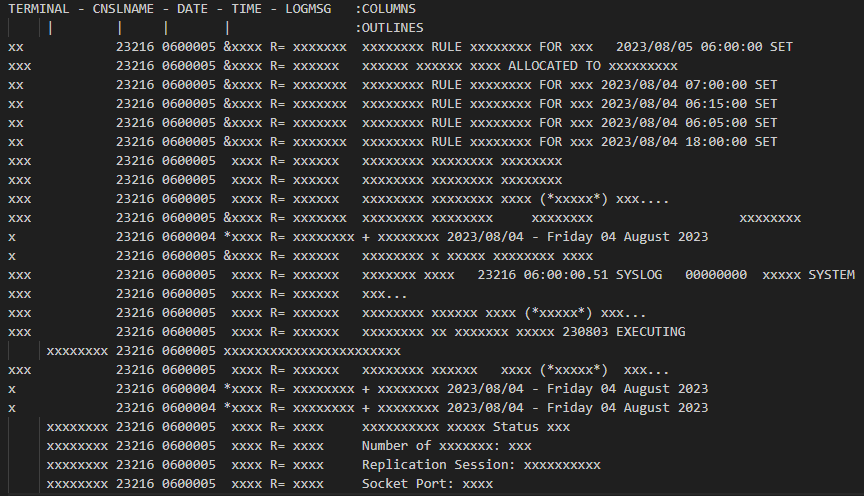
\includegraphics[width=1\linewidth]{bachproef/graphics/Voorbeeld_Syslog.png}
    \caption{Een voorbeeld van een SYSLOG met placeholdergegevens}
    \label{fig:Een voorbeeld van een SYSLOG met placeholdergegevens}
\end{figure}

Dit tekstbestand is per e-mail naar de verantwoordelijken voor de ELK-integratie van MFPOSS gestuurd. Daarbij is ook uitgelegd hoe het voorbeeld is opgebouwd. De eerste regel bevat alle kolomnamen. Daaronder staan regels die het begin van een nieuwe kolom vertegenwoordigen. Vanaf regel drie begint de log zelf. Nu de verantwoordelijken het bestand hebben ontvangen, kunnen ze doorgaan met het opzetten van ELK. Ze hadden ook enkele details nodig over enkele velden, zoals hoe de datum is opgebouwd uit twee tekens voor het jaar en drie tekens voor de dag van het jaar.

\subsection{Mockup}
Nadat een voorbeeld is verzonden, beschikken de verantwoordelijken over alle benodigde informatie om de ELK-integratie voor MFPOSS uit te voeren. Er volgden ook nog enkele vergaderingen waarin het ELK-team details wilde bespreken en bevestigen. Nu de ELK-integratie volop in gang is, kunnen we gelijktijdig beginnen met het ontwerpen van een mock-up voor het dashboard. Dit is het onderwerp van dit hoofdstuk. Op basis van de verwachtingen kunnen we concluderen dat MFPOSS een dashboard nodig heeft waarmee de volgende taken kunnen worden uitgevoerd via panelen:

1. Het bekijken van bepaalde logs.
2. Het detecteren van afwijkingen om te zien of er opvallende gebeurtenissen zijn opgetreden.
3. Mogelijk is er behoefte aan een plek voor documentatie.
4. Een grafiek met interessante gegevens, zoals de meest voorkomende logboekmelding.

\subsubsection{Probleem één}
Tijdens een van de vergaderingen met het ELK-team werd gevraagd naar afwijkingdetectie en wat de mogelijkheden waren om dit in een dashboard te integreren. Het blijkt dat de ELK-stack van Colruyt Group op dat moment nog geen afwijkingdetectie ondersteunt. Dit is een tekortkoming voor MFPOSS, maar het is geen reden om het onderzoek vroegtijdig te stoppen. Met deze nieuwe informatie kunnen we punt twee schrappen. Dit geeft ons ruimte om een andere grafiek toe te voegen.

\begin{figure}[h]
    \centering
    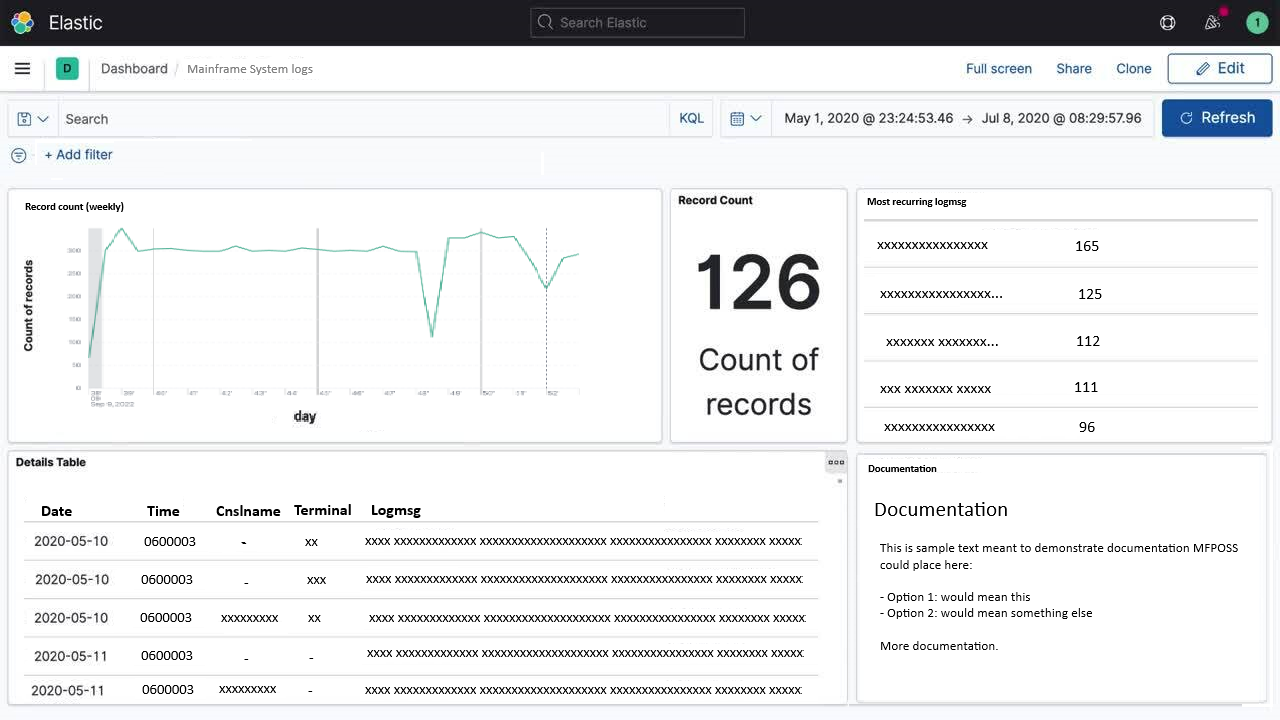
\includegraphics[width=1\linewidth]{bachproef//graphics/Dashboard_mockup.png}
    \caption{De mock-up voor het ELK-dashboard van MFPOSS}
    \label{fig: De mock-up voor het ELK-dashboard van MFPOSS}
\end{figure}

Figuur 4.3 is een mock-up van een dashboard dat mogelijk wordt verwacht. Het dashboard bestaat naast de Elastic-header uit vijf panelen. Er wordt hier natuurlijk gewerkt met fictieve gegevens die zo goed mogelijk echte gegevens proberen te representeren. Laten we kort de panelen bespreken. Het paneel op de eerste rij is een paneel met een lijngrafiek. Dit dient om te laten zien hoeveel regels de logs bevatten gedurende de afgelopen zeven dagen. Daarnaast is er een kleiner paneel dat snel het aantal regels weergeeft dat vandaag is ontvangen. Dit is handig om gemakkelijker te vergelijken met voorgaande dagen op de grafiek. Paneel drie is een lijst met de meest voorkomende regels. Een ervaren medewerker zou hier hopelijk al afwijkingen kunnen opmerken, aangezien afwijkingdetectie niet wordt gebruikt binnen Colruyt Group. Het tweede rij aan panelen bevat er twee: links de meest recente logs die ELK heeft ontvangen, en rechts een kader dat dient voor documentatie, tips of notities. Dit dashboard bevat al een groot deel van wat MFPOSS snel wil zien. Maar als men dieper in de gegevens wil kijken, is er ook de mogelijkheid om velden te doorzoeken en te visualiseren met behulp van de zoekbalk bovenaan.

\subsection{Versturen van data}
Naast de mock-up kunnen we ook kijken naar hoe gegevens naar ELK kunnen worden verzonden. Op verzoek van Dieter zal dit niet tijdens het onderzoek worden uitgevoerd, omdat dit te veel tijd kost door de betrokkenheid van een ander team dat verantwoordelijk is voor de planning van de taak. Het is ook niet noodzakelijk om de taak en planning gereed te hebben om het dashboard te maken en te analyseren. Voor het onderzoek zullen tien systeemlogs handmatig worden overgebracht naar het ELK-team, waarmee wordt gewerkt. Desondanks zal hier snel een voorbeeld worden besproken van een mogelijke taak, hoewel deze niet zal worden getest.

\begin{figure}[h]
    \centering
    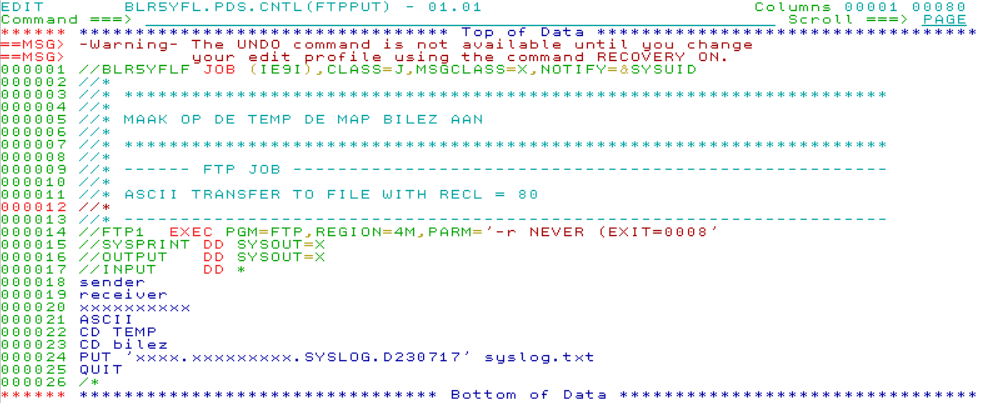
\includegraphics[width=1\linewidth]{bachproef//graphics/FTP JCL.png}
    \caption{Een voorbeeld van hoe een JCL-bestand voor FTP eruit kan zien}
    \label{fig:Een voorbeeld van hoe een JCL-bestand voor FTP eruit kan zien}
\end{figure}

Figuur 4.4 is een voorbeeld van een JCL-taak die bedoeld is om een bestand via FTP naar een bepaalde locatie te verzenden. Regel één is een standaard JCL-regel, waarbij de enige relevante variabelen de naam van de taak en het projectnummer zijn. Er zijn meer opties, maar die vallen buiten de reikwijdte van dit onderzoek. Regels twee tot en met dertien zijn opmerkingen. Regel veertien geeft aan dat dit een FTP-taak is. Vanaf regel achttien beginnen de variabelen en commando's om het bestand succesvol over te brengen:

\begin{itemize}
    \item lijn 18: De naam van het systeem dat het bestand verstuurt.
    \item lijn 19: De naam van het systeem dat het bestand ontvangt.
    \item lijn 20: Het wachtwoord van het ontvangende systeem.
    \item lijn 21: Het formaat van de inhoud van het bestand; voor dit onderzoek zou hoogstwaarschijnlijk voor ASCII worden gekozen.
    \item lijnen 22-23: Dit zijn commando's om naar de juiste directory te navigeren.
    \item lijn 24: Plaats het bestand van waar het is opgeslagen op het systeem dat verzendt naar de huidige locatie op het ontvangende systeem. Dit wordt gevolgd door de naam die het bestand moet hebben.
    \item lijn 25: Een commando om de FTP-sessie te beëindigen.
\end{itemize}

Een aangepaste versie van deze JCL-taak zou dan zijn verstrekt aan een team dat verantwoordelijk is voor de planning van taken om deze periodiek uit te voeren.
